%===========================================================
% This is the thesis template for the Statistics major at
% Amherst College. Brittney E. Bailey (bebailey@amherst.edu)
% adapted this template from the Reed College LaTeX thesis
% template in January 2019 with major updates in April 2020.
% Please send any comments/suggestions: bebailey@amherst.edu

% Most of the work for the original document class was done
% by Sam Noble (SN), as well as this template. Later comments
% etc. by Ben Salzberg (BTS). Additional restructuring and
% APA support by Jess Youngberg (JY). Email: cus@reed.edu
%===========================================================

\documentclass[12pt, twoside]{amherstthesis}
\usepackage{graphicx,latexsym}
\usepackage{amsmath}
\usepackage{amssymb,amsthm}
\usepackage{longtable,booktabs} %setspace loaded in .cls
\usepackage[hyphens]{url}
\usepackage{hyperref}
\usepackage{lmodern}
\usepackage{float}
\floatplacement{figure}{H}
\usepackage{rotating}
\usepackage{fancyvrb}
% User-added packages:
% End user-added packages

%===========================================================
% BIBLIOGRAPHY FORMATTING

% Next line commented out by CII
%%% \usepackage{natbib}
% Comment out the natbib line above and uncomment the
% following two lines to use the new biblatex-chicago style,
% for Chicago A. Also make some changes at the end where the
% bibliography is included.
%\usepackage{biblatex-chicago}
%\bibliography{thesis}


%===========================================================
% HYPERLINK FORMATTING

% Added by CII (Thanks, Hadley!)
% Use ref for internal links
\renewcommand{\hyperref}[2][???]{\autoref{#1}}
\def\chapterautorefname{Chapter}
\def\sectionautorefname{Section}
\def\subsectionautorefname{Subsection}
% End of CII addition
\usepackage{xcolor}
\hypersetup{
    colorlinks,
    linkcolor={red!50!black},
    citecolor={blue!50!black},
    urlcolor={blue!80!black}
}

%===========================================================
% CAPTION FORMATTING

% Added by CII
\usepackage{caption}
\captionsetup{width=5in}
% End of CII addition

%===========================================================
% TITLE FORMATTING

\renewcommand{\contentsname}{Table of Contents}

\usepackage{titlesec}
%%%%%%%%
% How to use titlesec:
% \titleformat{⟨command⟩}[⟨shape⟩]{⟨format⟩}{⟨label⟩}{⟨sep⟩}
%  {⟨before-code⟩}[⟨after-code⟩]
%%%%%%%%

\titleformat{\chapter}[hang]
{\normalfont%
    \Large% %change this size to your needs for the first line
    \bfseries}{\chaptertitlename\ \thechapter}{1em}{%
      %change this size to your needs for the second line
    }[]

\titleformat{\section}[hang]
{\normalfont%
    \large % %change this size to your needs for the first line
    \bfseries}{\thesection}{1em}{%
     %change this size to your needs for the second line
    }[]

\titleformat{\subsection}[hang]
{\normalfont%
    \normalsize % %change this size to your needs for the first line
    \bfseries}{\thesubsection}{1em}{%
     %change this size to your needs for the second line
    }[]

% \titleformat{\section}[display]
% {\normalfont%
%     \large% %change this size to your needs for the first line
%     \bfseries}{\chaptertitlename\ \thechapter}{20pt}{%
%     \normalsize %change this size to your needs for the second line
%     }


%===========================================================
% DOCUMENT FONT

% \usepackage{times}
% other fonts available eg: times, bookman, charter, palatino


%===========================================================
% PASSING FORMATS FROM RMD --> LATEX

%%%%%%%%
% NOTE: Dollar signs pass parameters between YAML inputs
% in index.Rmd and LaTeX
%%%%%%%%

\Abstract{
The abstract should be a short summary of your thesis work. A paragraph is usually sufficient here.
}

\Acknowledgments{
Use this space to thank those who have helped you in the thesis process (professors, staff, friends, family, etc.). If you had special funding to conduct your thesis work, that should be acknowledged here as well.
}

\Dedication{

}

\Preface{

}

% Formatting R code display
% Syntax highlighting #22

% Formatting R code: set baselinestretch = 1.5 for double-spacing
\DefineVerbatimEnvironment{Highlighting}{Verbatim}{
  baselinestretch = 1,
  commandchars=\\\{\}}

% Formatting R output display: set baselinestretch = 1.5 for double-spacing
\DefineVerbatimEnvironment{verbatim}{Verbatim}{
  baselinestretch = 1,
  % indent from left margin
  xleftmargin = 1mm,
  % vertical grey bar on left side of R output
  frame = leftline,
  framesep = 0pt,
  framerule = 1.5mm, rulecolor = \color{black!15}
  }

\title{Bayesian Nonparametric Regression Models for Quantifying Complex Interactions in Exposure Mixture Studies}
\author{Your R. Name}
\date{April DD, 20YY}
\division{}
\advisor{Advisor F. Name}
% for second advisor
\altadvisor{Your Other Advisor}
\institution{Amherst College}
\degree{Bachelor of Arts}
\department{Mathematics and Statistics}

% Fix from pandoc about cslreferences?
% https://github.com/mpark/wg21/issues/54
\newlength{\cslhangindent}
\setlength{\cslhangindent}{1.5em}
\newenvironment{CSLReferences}[2]%
  {}%
  {\par}

% Added by CII
%%% Copied from knitr
%% maxwidth is the original width if it's less than linewidth
%% otherwise use linewidth (to make sure the graphics do not exceed the margin)
\makeatletter
\def\maxwidth{ %
  \ifdim\Gin@nat@width>\linewidth
    \linewidth
  \else
    \Gin@nat@width
  \fi
}
\makeatother

% ===========================================
% DOCUMENT SPACING

\setlength{\parskip}{0pt}
% Added by CII

\providecommand{\tightlist}{%
  \setlength{\itemsep}{0pt}\setlength{\parskip}{0pt}}


% ===========================================
% ===========================================
% ===========================================
\begin{document}

\doublespace
% Everything below added by CII
  \maketitle

\frontmatter % this stuff will be roman-numbered
\pagenumbering{roman}
\pagestyle{fancyplain}
%\pagestyle{fancy} % this removes page numbers from the frontmatter

  \begin{abstract}
    The abstract should be a short summary of your thesis work. A paragraph is usually sufficient here.
  \end{abstract}
  \begin{acknowledgments}
    Use this space to thank those who have helped you in the thesis process (professors, staff, friends, family, etc.). If you had special funding to conduct your thesis work, that should be acknowledged here as well.
  \end{acknowledgments}

  \hypersetup{linkcolor=black}
  \setcounter{tocdepth}{2}
  \tableofcontents

  \addcontentsline{toc}{chapter}{List of Tables}\listoftables

  \addcontentsline{toc}{chapter}{List of Figures}\listoffigures


\mainmatter % here the regular arabic numbering starts
\pagenumbering{arabic}
\pagestyle{fancyplain} % turns page numbering back on

\hypertarget{intro}{%
\chapter{Introduction}\label{intro}}

Rapid industrial development has created conditions of cumulative chronic toxicity which pose an acute risk to the wellbeing of humans and our living environment. It has been estimated that human activity releases chemicals at a rate of 220 billion tons per annum (Cribb, 2016). Scholars have recently formally declared that, at this global rate of chemical release, humanity has surpassed the safe operating space of the planetary boundary for novel entities (Persson et al., 2022). As a result, exposure to low levels of pollutants has become an inevitable peril of daily life (Naidu et al., 2021; Vineis, 2018). Hence, it is especially timely that we prompt regulatory control of industrial pollution through studies which investigate the health effects of chemical exposures.

For this, we turn to epidemiological studies. The broad field of preventive epidemiology involves the identification of potentially modifiable risk factors that contribute to the burden of disease within human populations. Environmental epidemiology, in particular, considers the effect of environmental exposures --- chemical or otherwise. However, studies concerning chemical pollutants in environmental epidemiology have historically focused on elucidating the effect and mechanisms of exposures to a single pollutant. In reality, humans are invariably exposed to numerous complex chemical mixtures which together contribute to the progression of adverse health outcomes. Therefore, risk assessments of single pollutants likely fail to capture the true consequences of these complex exposures (Heys et al., 2016). Assessing mixtures of chemicals can also have more direct implications for public health interventions. The United States Environmental Protection Agency (U.S. EPA) currently passes regulations for individual pollutants. In practice, though, regulation occurs by controlling the source of pollution, which is responsible for the production of a whole mixture of chemicals with specific joint effects on human health. As a result, the National Academies of Science has advocated for a multipollutant regulatory approach, which is likely to be more protective of human health (Committee on Incorporating 21st Century Science into Risk-Based Evaluations et al., 2017).

There are clear practical motivations for studies that examine the health effects of exposure to co-occurring chemical mixtures, hereafter referred to as exposure mixtures. However, expanding the focus of analysis from one exposure to multiple exposures introduces unique statistical challenges. In addition to a common issue of small effect sizes and small sample sizes present in most exposure analyses, multiple exposure analyses must also contend with high-dimensionality, collinearity, non-linear effects, and non-additive interactions (Yu et al., 2022). In particular, data with numerous pollutants, or predictors, require exponentially greater levels of complexity and time cost in analysis. Collinearity between exposures is common when analyzing pollutants from a single source and can lead to unstable estimates in a generalized linear model if left unaccounted for. Finally, exposures can have both non-linear single effects and non-additive interaction effects, which are difficult to capture unless explicitly specified in the model.

The classic multiple linear regression framework often fails to capture the true effects in this setting. In the past few years, a wide variety of statistical methods have been developed to overcome these challenges (Gibson et al., 2019; Yu et al., 2022), which have been accompanied by a host of comparative simulation studies for general mixture scenarios (e.g., Hoskovec et al., 2021; Lazarevic et al., 2020; Pesenti et al., 2023). However, there is not yet conclusive guidance about the ability of these methods to conduct inference on non-additive interactions between exposures.

The goal of this thesis is to fill this gap in the literature by exploring the theory and performance of Bayesian regression techniques for quantifying complex interactions between environmental exposures. Specifically, I will compare two recently developed models for estimating the health effects of exposure mixtures: Bayesian Kernel Machine Regression (BKMR, Bobb et al., 2015) and Bayesian Semiparametric Regression (BSR, Antonelli et al., 2020).

In an age where anthropogenic actions have radically reshaped the earth, humanistic inquiry can offer critical insights into how we navigate the hazards of our rapidly changing environment. I begin in Chapter 2 by contextualizing this thesis with a brief overview of cultural and social understandings of toxicity. Chapter 3 explains the motivation for studying interactions and provides background on the theory of Bayesian methods for analyzing exposure mixtures. Chapter 4 assesses the performance of these methods using a simulation study, based on a dataset with information on the relationship between prenatal exposure to heavy metals and gestational weight. Chapter 5 explores an application on X data {[}TBD{]}. I conclude with a discussion of the implications of this work for the future study of complex interactions in exposure mixture studies.

\hypertarget{humanistic}{%
\chapter{Humanistic perspective}\label{humanistic}}

\hypertarget{bayes}{%
\chapter{Bayesian regression methods}\label{bayes}}

\hypertarget{motivation}{%
\section{Motivation}\label{motivation}}

We are interested in using Bayesian regression techniques to characterize the nature of complex interactions. In addition to being an interesting statistical challenge, complex interactions are also relevant from both a mechanistic and public health point of view.
\begin{itemize}
\tightlist
\item
  mechanistic
\item
  public health
\end{itemize}
Drawing from the mechanistic and public health contexts, there are three classes of interactions that are of interest.
\begin{itemize}
\tightlist
\item
  different types of interactions
\end{itemize}
However, non-additive interactions are difficult to detect.

First, there are different forms that an interaction can take on. For instance, in the linear regression setting, the form of the interaction must be explicitly specified; most commonly, this is done by multiplying two variables together. However,

Moreover, the number of possible interactions to consider quickly becomes intractable in high-dimensional settings. For instance, consider modelling 10 exposures in a linear regression setting. In order to be assessed, each interaction must be explicitly specified as a new term in the model. Including all the possible two-way interactions would involve adding \({10 \choose 2} = 45\) additional terms to the model, and all possible three-way interactions would add \({10 \choose 3} = 120\) additional terms.
\begin{itemize}
\tightlist
\item
  interactions are difficult to pick up
\item
  consider the number of interactions that would have to be encoded explicitly in MLR
\end{itemize}
It is important also to acknowledge, here, that there is a limit to how many variables can be included in an interaction before it becomes incomprehensible to most humans.

\hypertarget{bayesian-kernel-machine-regression}{%
\section{Bayesian kernel machine regression}\label{bayesian-kernel-machine-regression}}

Defining notation:
\begin{itemize}
\tightlist
\item
  observations from \(i = 1, \dots ,n\)
\item
  \(\textbf{x}_m\) is a predictor variable in the predictor matrix \(\textbf{X}\) with \(m = 1, \dots, M\), measuring exposure variables in this case
\item
  \(\textbf{x}_i\) is a vector of values for a single observation in \(\textbf{X}\) with \(i = 1, \dots, n\), measuring the health outcome in this case
\item
  \(x_{im}\) is an observation of \(\textbf{x}_m\)
\item
  \(Y_i\) is an observation of \(\textbf{Y}\)
\item
  \(\rho\) is the tuning parameter inside the exponential expression of the covariance, equals \(2l\)
\item
  \(\tau\) is the tuning parameter outside the expontential expression of the covariance, equals \(\sigma_f^2\)
\item
  \(k\) is the smoothing function, the Gaussian in this case
\item
  \(\textbf{K}\) is the \(n \times n\)kernel matrix, with (i, j)th element \(k(\textbf{x}_i, \textbf{x}_j)\)
\item
  \(h(\textbf{x}_i)\) the flexible function relating X to Y
\item
  \(\boldsymbol\epsilon_i \overset{\mathrm{iid}}{\sim} N(0, \sigma^2)\), the residuals of the response
\end{itemize}
\hypertarget{kernel-machine-regression}{%
\subsection{Kernel machine regression}\label{kernel-machine-regression}}

In this section, we introduce kernel machine regression, with attention to its specific implementation in BKMR. Kernel machine regression is a nonparametric regression technique that can be used to capture nonlinear effects and nonadditive interactions. In the typical linear regression setting,

\[
Y_i = \textbf{x}_i^\top\boldsymbol{\beta} + \epsilon_i
\]

\noindent where \(Y_i\) measures a health outcome at a given point, \(\textbf{x}_i = (x_{1},\dots,x_{M})^\top\) is a vector of M exposures, \(\boldsymbol{\beta}\) is a vector of weights, and \(\epsilon_i\) is a random variable from \(\boldsymbol\epsilon \overset{\mathrm{iid}}{\sim} N(0, \sigma^2)\). We can see that this function assumes that there is a linear relationship between the exposure and the response, and that the combined effects of multiple exposures are additive.

Kernel machine regression defines this relationship using a function \(h: \mathbb{R}^M \rightarrow \mathbb{R}\), where

\[
Y_i = h(\textbf{x}_i) + \epsilon_i
\]

\noindent Here, \(h(\cdot)\) is represented by the function \(k(\cdot, \cdot)\), a kernel. The kernel controls the covariance, or the similarity, between values of \(h(\textbf{x})\) and as such ensures that points near each other on the prediction surface will have similar values --- or, in other words, that the prediction surface will be smooth. In the case of kernel machine regression, we define a positive definite kernel where \(k: \mathbb{R}^M\times \mathbb{R}^M \rightarrow \mathbb{R}\). There are many choices of functions to represent \(k\). BKMR uses the Gaussian kernel, also known as the radial basis function or, sometimes, the squared exponential kernel. The Gaussian kernel is defined

\[
k(\textbf{x}, \textbf{x}') = \sigma_f^2\textrm{exp}\{
-\frac{||\textbf{x}-\textbf{x}'||^2}{2l}\}
\]

\noindent where \(||\textbf{x}-\textbf{x}'||^2 = \sum_{m=1}^M{(x_{m}-x_{m}')^2}\) for \(\textbf{x}\), a set of exposure values, and \(\textbf{x}\), the exposure profile of a second subject, \(\sigma_f^2\) is a tuning parameter that controls how much the function is allowed to vary, and \(l\) is a tuning parameter that controls the relationship between the correlation between two points and their distance. Greater values of \(l\) will enforce more dependence between points and make the resulting function smoother. Note that BKMR uses \(\rho=2l\) and \(\tau=\sigma_f^2\), so, henceforth, we will be referring to these parameters using BKMR's notation.

Now that we have defined \(h\) and \(k\), we can think about how to characterize the relationship between our response and predictors. Kernel machine regression is a nonparametric technique because it does not specify a functional form for this relationship. Hence, we will think about estimating the response at a particular query point. Operationally, kernel machine regression uses a weighted average of all the observations in the dataset to estimate the response, as follows

\[
\bar{Y} = \frac{\sum_{i=1}^nw_iY_i}{\sum_{i=1}^nw_i}
\]

\noindent with some set of weights \(\{w_i\}_{i=1}^n\). Intuitively, we want to weight the observations that are closer to the query point more heavily. Using the Gaussian kernel as a weight allows us to achieve this. Replacing the weight with the Gaussian kernel, we get

\[
\bar{Y} = \frac{\sum_{i=1}^n K(\textbf{x}, \textbf{x}_i) Y_i}
{\sum_{i=1}^n K(\textbf{x}, \textbf{x}_i)}
\]

As we move through the predictor space, we can think of the prediction as a continuous moving average of local points in the dataset. This gives us the following relationship

\[
\textrm{cor}(h_i, h_j) = \textrm{exp}\{-(\frac{1}{\rho}) \sum_{m=1}^M
{(x_{im}-x_{jm})^2}\}
\]

\noindent which allows us to see that values \(h\) near each other will have a higher correlation and thus similar values. This is also why the resulting function is smooth.

\hypertarget{connection-with-mixed-models}{%
\subsection{Connection with mixed models}\label{connection-with-mixed-models}}

It is useful to make connections between this definition of kernel machine regression and mixed models. To do this, we can represent \(h(\textbf{x})\) as following a Gaussian process probability distribution, defined

\[
h(\textbf{x}) \sim \mathcal{GP}(\textbf{0}, k(\textbf{x}, \textbf{x}'))
\]

\noindent with mean function \(m\) and covariance function \(k\), where \(\textbf{x}\) is a vector of exposure values, and \(\textbf{x}'\) is the exposure profile of another subject. A Gaussian process is a collection of random variables, of which any finite number follow a multivariate normal distribution. Here, we assume that the expected value of the function with input \(\textbf{x}\) is \(\textbf{0}\). We use \(k\) for the covariance function, which represents the dependence between the function values with inputs \(\textbf{x}\) and \(\textbf{x}'\): \(k(\textbf{x}, \textbf{x}') = \mathbb{E}[(h(\textbf{x})-m(\textbf{x})) (h(\textbf{x}')-m(\textbf{x}'))]\).

Now, we can represent \(h\) as a collection of variables from a Gaussian process. \(h\) follows a multivariate normal distribution

\[
h({\textbf{x}}) \sim N(\textbf{0}, \textbf{K})
\]

\noindent where \(h({\textbf{x}}) = h(\textbf{x}_1), h(\textbf{x}_2), \dots, h(\textbf{x}_n)\), and \(\textbf{K}\) is the kernel matrix. The kernel matrix is an \(n \times n\) matrix with \((i, j)\)th element \(k(\textbf{x}_i, \textbf{x}_j)\). Now, returning back to the regression view, we can think of each \(Y_i\) as following the distribution

\[
Y_i \overset{\mathrm{ind}}{\sim} N(h(\textbf{x}_i), \sigma^2) \text{ for } i = 1,\dots,n
\]

\noindent where \(\sigma^2\) comes from the variance of the residuals.

\hypertarget{toy-example}{%
\subsection{Toy example}\label{toy-example}}

In the following section, we introduce the technique with a toy example.

Consider the following case where we want to model the relationship between a single predictor and a response variable. Suppose the true relationship between x and Y is defined \(Y = e^{\frac{x}{10}} + 2\sin(\frac{x}{2})\)
\begin{center}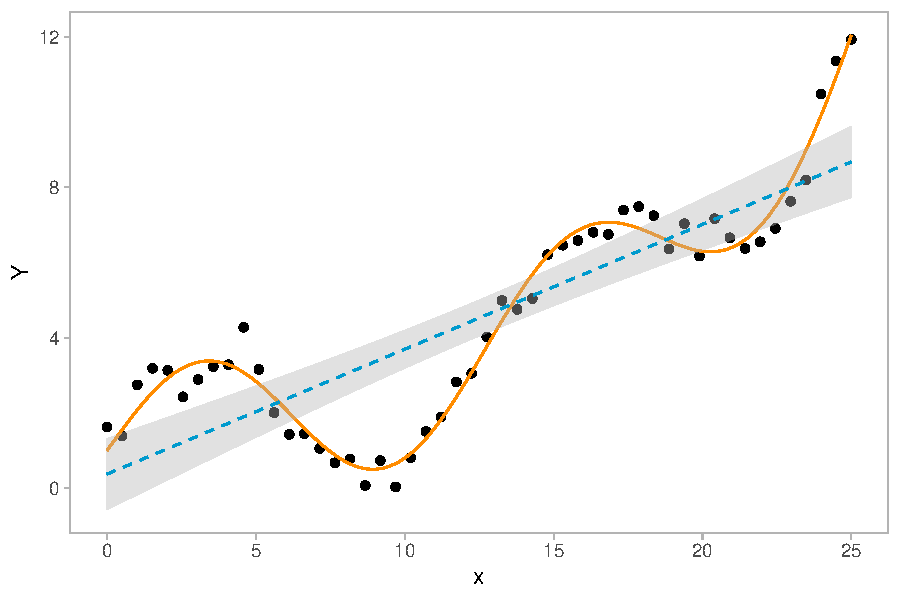
\includegraphics{Elizabeth-Zhang_StatThesis_files/figure-latex/unnamed-chunk-2-1} \end{center}

Define a query point
\begin{center}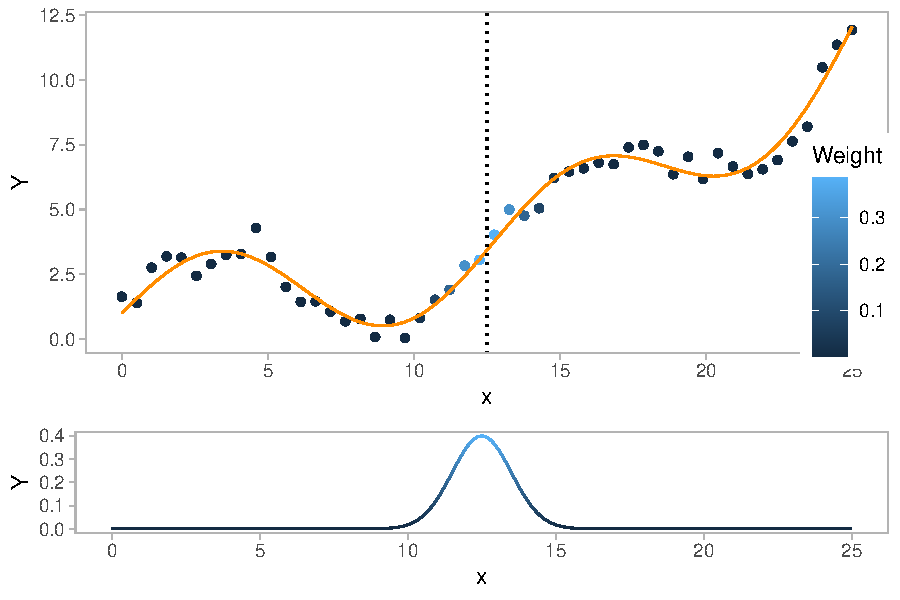
\includegraphics{Elizabeth-Zhang_StatThesis_files/figure-latex/unnamed-chunk-3-1} \end{center}

Note to self, bandwidth represent four times the quartiles of the probability density. In the case of a Gaussian kernel, the bandwidth represents \(\frac{8}{3}\sigma\), so using an sd of 1 translates to bandwidth of 8/3
\begin{center}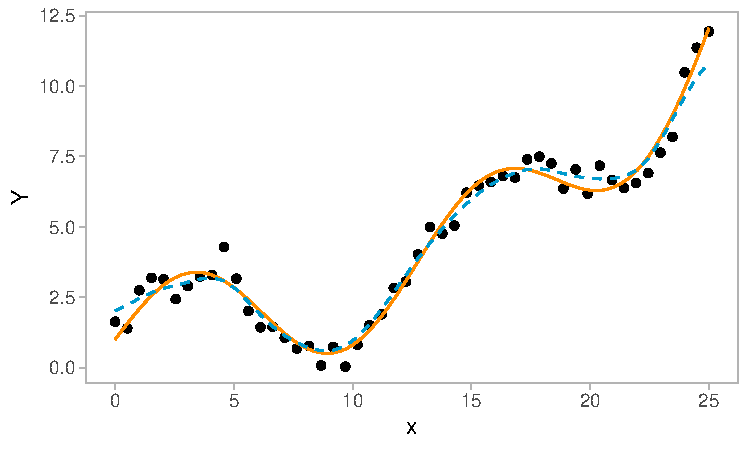
\includegraphics{Elizabeth-Zhang_StatThesis_files/figure-latex/unnamed-chunk-4-1} \end{center}

We can also use this example to understand how our choice of the scaling parameter influences model fit.

\hypertarget{variable-selection}{%
\subsection{Variable selection}\label{variable-selection}}

In this section, we discuss the two methods for variable selection in BKMR: hierarchical variable selectiona and component-wise variable selection.

\hypertarget{priors-in-a-bayesian-framework}{%
\subsection{Priors in a Bayesian framework}\label{priors-in-a-bayesian-framework}}

Discuss priors, what form do they take? what are the default settings?

\hypertarget{the-mcmc-algorithm}{%
\subsection{The MCMC algorithm}\label{the-mcmc-algorithm}}

Brief intro to MCMC

\hypertarget{detecting-interactions}{%
\subsection{Detecting interactions}\label{detecting-interactions}}

Discuss options for detecting interactions, i.e., can visualize relationship at various quantiles of other predictor, can conduct inference on inter-quantile difference

Potentially provide toy example

\hypertarget{bayesian-semiparametric-regression}{%
\section{Bayesian semiparametric regression}\label{bayesian-semiparametric-regression}}

differences w/ bkmr
\begin{itemize}
\tightlist
\item
  makes distributional assumptions about the dataset
\item
  kernel regression is computationally intensive w/ large datasets but can handle many predictors
\item
  bsr highly dependent on the choice of function
\end{itemize}
\hypertarget{connections-to-linear-mixed-model}{%
\subsection{Connections to linear mixed model}\label{connections-to-linear-mixed-model}}

\hypertarget{toy-example-1}{%
\subsection{Toy example}\label{toy-example-1}}
\begin{center}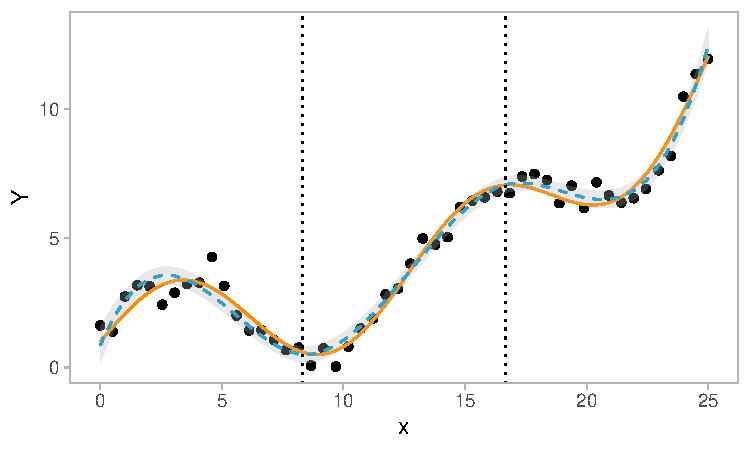
\includegraphics{Elizabeth-Zhang_StatThesis_files/figure-latex/unnamed-chunk-5-1} \end{center}

--\textgreater{}

\hypertarget{sims}{%
\chapter{Simulations}\label{sims}}

\hypertarget{past-simulation-studies}{%
\section{Past simulation studies}\label{past-simulation-studies}}

\hypertarget{madres-data}{%
\section{MADRES data}\label{madres-data}}

\hypertarget{conclusion}{%
\chapter*{Conclusion}\label{conclusion}}
\addcontentsline{toc}{chapter}{Conclusion}

If we don't want the conclusion to have a chapter number next to it, we can add the \texttt{\{-\}} attribute.

\textbf{More info}

And here's some other random info: the first paragraph after a chapter title or section head \emph{shouldn't be} indented, because indents are to tell the reader that you're starting a new paragraph. Since that's obvious after a chapter or section title, proper typesetting doesn't add an indent there.

\appendix

\hypertarget{the-first-appendix}{%
\chapter{The First Appendix}\label{the-first-appendix}}

This first appendix includes all of the R chunks of code that were hidden throughout the document (using the \texttt{include\ =\ FALSE} chunk tag) to help with readibility and/or setup.

\hypertarget{in-the-main-file-refref-labels}{%
\section{In the main file \ref{ref-labels}:}\label{in-the-main-file-refref-labels}}

\hypertarget{in-chapter-refref-labels}{%
\section{In Chapter \ref{ref-labels}:}\label{in-chapter-refref-labels}}

\hypertarget{the-second-appendix}{%
\chapter{The Second Appendix}\label{the-second-appendix}}

R code

\hypertarget{corrections}{%
\chapter*{Corrections}\label{corrections}}
\addcontentsline{toc}{chapter}{Corrections}

A list of corrections after submission to department.

Corrections may be made to the body of the thesis, but every such correction will be acknowledged in a list under the heading ``Corrections,'' along with the statement ``When originally submitted, this honors thesis contained some errors which have been corrected in the current version. Here is a list of the errors that were corrected.'' This list will be given on a sheet or sheets to be appended to the thesis. Corrections to spelling, grammar, or typography may be acknowledged by a general statement such as ``30 spellings were corrected in various places in the thesis, and the notation for definite integral was changed in approximately 10 places.'' However, any correction that affects the meaning of a sentence or paragraph should be described in careful detail. The files samplethesis.tex and samplethesis.pdf show what the ``Corrections'' section should look like. Questions about what should appear in the ``Corrections'' should be directed to the Chair.

\backmatter

\hypertarget{references}{%
\chapter*{References}\label{references}}
\addcontentsline{toc}{chapter}{References}

\noindent

\setlength{\parindent}{-0.20in}
\setlength{\leftskip}{0.20in}
\setlength{\parskip}{8pt}

\hypertarget{refs}{}
\begin{CSLReferences}{1}{0}
\leavevmode\vadjust pre{\hypertarget{ref-angel2000}{}}%
Angel, E. (2000). \emph{Interactive computer graphics : A top-down approach with OpenGL}. Boston, MA: Addison Wesley Longman.

\leavevmode\vadjust pre{\hypertarget{ref-angel2001}{}}%
Angel, E. (2001a). \emph{Batch-file computer graphics : A bottom-up approach with QuickTime}. Boston, MA: Wesley Addison Longman.

\leavevmode\vadjust pre{\hypertarget{ref-angel2002a}{}}%
Angel, E. (2001b). \emph{Test second book by angel}. Boston, MA: Wesley Addison Longman.

\end{CSLReferences}
% Index?

\end{document}
